\documentclass[10pt]{article}
\usepackage[a4paper,margin=17mm]{geometry}\usepackage[T1]{fontenc}
\usepackage{lmodern,amsmath,amssymb,graphicx,booktabs,hyperref}
\setlength{\parindent}{0pt}\setlength{\parskip}{5pt}\sloppy\setlength{\emergencystretch}{3em}
\begin{document}
\begin{center}{\Large First full native run: successful, receipt label corrected}\\cm8-dual-20261029\end{center}
The first complete native contract passes14+14points,392addition pairs,7subgroup
inverses,all12S3arms/72recoveries,9changed/rehashed controls and22backend tests.
The receipt originally named rejected valid points ``nontorsion''. All finite
group points are torsion; the actual seven points are not killed by7. Source
correction changes only that JSON key, with full second replay. Original source
and successful output remain. This first run is not a failure and is not erased.
No timing, useful-yield change or total-cost gain was admitted.
\par
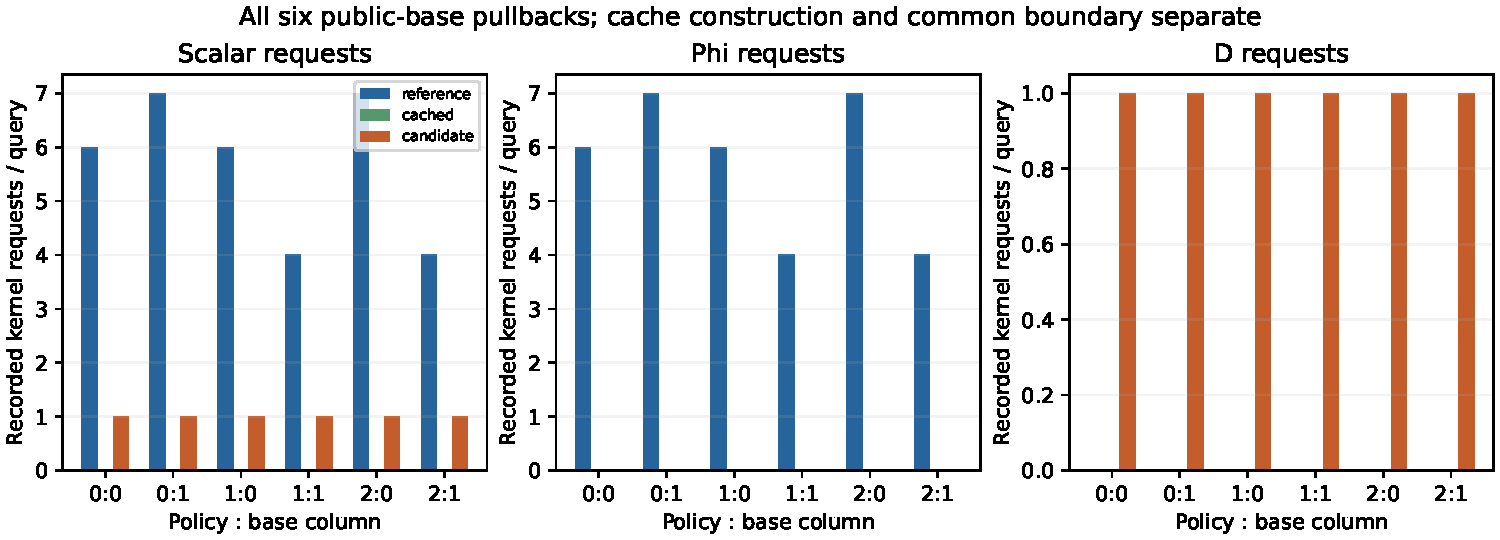
\includegraphics[width=\linewidth]{../requests.pdf}\par
Full report: \path{reports/cm8-dual-20261029/README.md}. Exact command/source/logs:
\path{validation/cm8-dual-20261029/restore-runs.sh}. Existing local resources,
600sec caps, no paid compute, no new general geometric-duality/speed claim.
\end{document}
